% Created 2018-02-21 Wed 19:30
% Intended LaTeX compiler: pdflatex

\documentclass[twocolumn,twoside]{IEEEtran}
% \documentclass[journal,twocolumn,twoside]{IEEEtran}
% \documentclass[journal,12pt,onecolumn,draftclsnofoot,,twoside]{IEEEtran/IEEEtran}
\pdfminorversion 4 % This is so manuscript central can use it.

% \usepackage[utf8]{inputenc}
% \usepackage[T1]{fontenc}
% \usepackage{grffile}
% \usepackage{rotating}
% \usepackage[normalem]{ulem}
% \usepackage{hyperref}
% \usepackage{textcomp}
% \usepackage{capt-of}

\usepackage[table,dvipsnames]{xcolor}

\usepackage{graphicx}
\usepackage{cite} % Need this to get compressed citation, e.g., [4]-[7]
\usepackage{longtable}
\usepackage{wrapfig}

\usepackage{booktabs}
\usepackage{amsmath}
\usepackage{amssymb}
\usepackage{mathtools}
% \mathtoolsset{showonlyrefs=true}
\usepackage[inkscapelatex=false, inkscapepath=svgsubpath]{svg}
\usepackage{subcaption}
\usepackage{xspace, dsfont}
\usepackage{mathtools}
\usepackage{multirow}
\usepackage{overpic}
% \usepackage[table]{colortbl}

\usepackage[textsize=tiny,textwidth=1\marginparwidth,draft,obeyFinal]{todonotes}

\usepackage{courier} %for fixed-width, \texttt{stuff}
\newcommand{\Dm}{\ensuremath{\mathcal{D}_{-} }\xspace}
\newcommand{\U}{\ensuremath{\mathcal{U} }\xspace}
\newcommand{\DU}{\ensuremath{\Delta \mathcal{U} }\xspace}
\newcommand{\Q}{\ensuremath{\mathcal{Q} }\xspace}
\newcommand{\R}{\ensuremath{\mathcal{R} }\xspace}
\newcommand{\Hh}{\ensuremath{\mathcal{H} }\xspace}
\newcommand{\du}{\ensuremath{\Delta u }\xspace}
\newcommand{\dU}{\ensuremath{\Delta \mathcal{u} }\xspace}
\newcommand{\Gd}{\ensuremath{\bar G }\xspace}
\newcommand{\Ad}{\ensuremath{\bar A }\xspace}
\newcommand{\Bd}{\ensuremath{\bar B }\xspace}
\newcommand{\Cd}{\ensuremath{\bar C }\xspace}
\newcommand{\xd}{\ensuremath{\bar x }\xspace}
\newcommand{\Qd}{\ensuremath{\bar Q }\xspace}
\newcommand{\Rd}{\ensuremath{\bar R }\xspace}
\newcommand{\x}{\ensuremath{x }\xspace}
\newcommand{\xdss}{\ensuremath{\bar x_{ss} }\xspace}
\newcommand{\xde}{\ensuremath{\bar x_{e} }\xspace}
\newcommand{\xo}{\ensuremath{\hat x }\xspace}
\newcommand{\yr}{\ensuremath{y_{r} }\xspace}
\newcommand{\y}{\ensuremath{y} \xspace}
\newcommand{\dd}{\ensuremath{\Delta }\xspace}
\newcommand{\Gv}{\ensuremath{G_{\text{vib}}}\xspace}
\newcommand{\hGv}{\ensuremath{\hat{G}_{\text{vib}}}\xspace}

% \newcommand{\ub}{\ensuremath{\bar{u} }\xspace}
% \newcommand{\ubp}{\ensuremath{\bar{u}^+ }\xspace}
% \newcommand{\ubm}{\ensuremath{\bar{u}^- }\xspace}


\begin{document}
\title{A Comparison of Tracking Step Inputs with a Piezo Stage Using MPC and Saturated LQG Control}
  % Control strategies for step tracking a piezo stage}
\author{Roger A. Braker and Lucy Y. Pao
  \thanks{The authors are with the Dept. of Electrical, Computer, and Energy Engineering at the University of Colorado, 425 UCB, Boulder, CO 80309, United States. Phone: +1 (303) 492-2360. Fax: +1 (303) 492-2758.
    R. A.  Braker (corresponding author roger.braker@colorado.edu) is a graduate student and
    L.Y. Pao (pao@colorado.edu) is the Palmer Endowed Professor.}
  \thanks{This work was supported in part by the US National Science Foundation (NSF Grant CMMI-1234980), Agilent Technologies, Inc., and the Hanse Wissenschaftskolleg in Delmenhorst, Germany.}
}

\maketitle
\begin{abstract}
  Compressed Sensing for Atomic Force Microscopy is a newer imaging mode that requires the piezo stage be driven rapidly between measurement locations. In contrast to raster scanning applications, this translates to a setpoint tracking problem. 
  This paper considers the setpoint tracking performance of a piezo nano-positioning stage subject to rate-of-change limitations on the control signal, which we derive from the current limit of the power amplifier.
To compensate the vibrational dynamics of the stage, we consider a model predictive control scheme and an LQG controller which saturates the control increment. In both cases, hysteresis and drift are compensated via dynamic inversion. We analyze the robustness of both schemes using classical methods. We conclude that model predictive control is of limited practical utility because selecting the control weights such that model predictive control is nominally beneficial results in degraded robustness, and thus in poor experimental performance.
\end{abstract}


\section{Introduction}\label{sec:intro}
The Atomic Force Microscope (AFM) is a nano-scale imaging instrument which acquires an image of the surface topography of a sample by mechanically interrogating it with an atomically-sharp probe \cite{abramovitch_tutorial_2007, rana_improvement_survey_2017}. Typically, the probe is scanned across a specimen in a raster pattern, sequentially acquiring pixels in an image. Although this process gives the AFM excellent spatial resolution, the serial acquisition of pixels limits the speed of any given instrument, yielding frame rates on the order of minutes for many commercially available instruments.

While slow imaging is inconvenient for static samples, it represents a fundamental limitation in the study of dynamic specimens. Many methods have been proposed to increase AFM frame rates, including better mechanical design~\cite{schitter_designmodeling,kenton_threeaxis}, using advanced control methods~\cite{butterworth_dualadaptive_2011, li_feedforward_2007, Leang_IEEECS_2009, reza_zaxis_videorate}, and alternative scanning methods \cite{Mahmood_nano_2009,Tuma_highspeed_2012,rana_spiral_2014,fleming_bridging_2010, Huang_fast_2014,Hartman_feature_2017}.

One newer alternative to raster scanning, and which is our interest here, is the application of Compressive Sensing to AFM~\cite{oxvig_structure_2017, andersson_pao, song_video_2011}. The central idea of compressive-sensing-based imaging is to leverage the redundancy present in most interesting signals such that the  number of pixels to be acquired is reduced. For good guarantees on reconstruction quality, measurements in compressive-sensing-based imaging need to be randomly distributed across the specimen. Each measurement might acquire a single pixel \cite{andersson_pao} or short string of adjacent pixels in a micro-scan \cite{braker_hardware_2018, maxwell_acc_2014}. Once a measurement is completed, the AFM probe is retracted from the sample surface,  moved in the XY plane to the next measurement location and finally re-engaged with the specimen surface before the next measurement is acquired. Details of a basic implementation of this approach can be found in \cite{braker_hardware_2018}.

In this paper we are concerned with the point-to-point movement in the XY plane between measurement locations. During this operation, the probe is not in contact with the specimen. Thus, it is desirable to minimize the time to move between measurement locations. Thus, in contrast to standard raster scanning where the control goal is to minimize overall tracking error to a triangular reference, the goal here is to minimize the settling time to a step input. Point-to-point movements by AFM are also of interest in other areas like visceolastic property mapping \cite{killgore_visceolastic_2011}.

\begin{figure*}
  \centering
  % [grid]
  \begin{overpic}[scale=1]{figures/blocks/ss_block_diagram_cropped.pdf}
    \put(54.5,19){$\hat{G}_d${\raisebox{1.15ex}{$\scriptscriptstyle -1$}} }
    \put(63.,19){$\mathcal{F}${\raisebox{1.15ex}{$\scriptscriptstyle -1$}}$[\cdot]$}
    \put(76.4,19){$\mathcal{F}[\cdot]$}
% \includegraphics                
\end{overpic}
  \caption{The overall plant model consists of a hysteresis model $\mathcal{F}[\cdot]$,  a drift model $G_{d}$, and a vibrational model $\Gv$. The effects of drift and hysteresis are compensated for via dynamic inversion.}
  \label{fig:ss_bd}
\end{figure*}

One of the primary constraints in setpoint tracking with our piezo stage is the current limit of the power amplifier,  which roughly translates to a slew-rate limitation on the control signal.
In principle, minimizing the settling-time of such point-to-point motions is a classic time-optimal control problem. % For piezo stages which can be adequately modeled as a second-order system, we have considered robust methods to effect this \cite{braker_proximate_2017}. 
However, for stages with dynamics more complex than a second-order system,  including the stage in our own lab, closed-form solutions to the minimum-time problem are intractable. 

An enticing alternative to explicitly handle the slew-rate constraint is MPC with a purely quadratic cost. 
Given a discrete-time state-space system $\{A,B,C,0\}$ with state $x_k$, and control input $u_k$, such an MPC scheme solves, at each time step, the optimal control problem 
\begin{subequations}
\begin{align}
\min_{v}\:\:& z^T_{N}Pz_{N} + \sum_{i=0}^{N-1}z_{i}^{T}Qz_{i} + 2z^T_iSv_i + v^{T}_{i}Rv_{i} \\
 \text{s.t.} \quad z_{i+1} &= A z_{i} + B v_{i}\\
z_{0} &= x_{k}, \\
v_i  &\in \mathds{U} \label{eqn:ucon0}
\end{align}\label{eqn:optcost0}%
\end{subequations}
where $\mathds{U}$ is a polyhedron, $P$ solves the Discrete Algebraic Riccati Equation (DARE), $Q$ and $R$ are symmetric matrices and, together with $S$, satisfy
\begin{align}
  R &> 0 \label{eqn:schur0}\\
  Q - SR^{-1}S^T &\geq 0. \label{eqn:schur1}
\end{align}
% \begin{equation}
%   \begin{bmatrix}
%     Q & S\\S^T &R
%   \end{bmatrix} > 0.
% \end{equation}
In this paper, we restrict $\mathds{U}$ to model actuator constraints (e.g., saturation). The solution to the quadratic program (QP) \eqref{eqn:optcost0} results in a sequence of optimal controls $v_0\dots v_{N-1}$. One sets $u_k = v_0$ and repeats the process at the next time step. If one eliminate the constraint \eqref{eqn:ucon0}, then the control action reduces to linear state-feedback. That is, $v_0=-Kx_k$ where
\begin{equation}
  K = (\Bd^TP\Bd + R)^{-1}(\Bd^TP\Ad + S^T),\label{eqn:klin0}
\end{equation}
is the solution to the infinite horizon LQR problem associated with $Q$, $R$ and $S$. 

Historically, one of the challenges of applying MPC to systems with fast dynamics is the computational demand imposed by solving a QP within a small sample period. However, advances in both hardware and algorithms have mitigated this issue. For example, \cite{Jerez_Trans_2014} shows that when $\mathds{U}$ is a simple box (i.e., a saturating constraint), sample rates of up to 1 MHz can be achieved with high-end FPGAs using an algorithm called the Fast Gradient Method (FGM). 

% The classical alternative to MPC with respect to constraint violation is to simply relax the performance criteria, e.g., by increasing the control weight and instituting a linear feedback law. Because MPC is considerably more difficult to implement and requires more computation time and/or hardware resources compared to linear feedback, an important question is  ``how much \emph{time} is actually saved with MPC?"
% % Explorations following this line of reasoning have not seen much attention in the applied MPC literature.

In recent work, we applied the FGM formulation of \cite{Jerez_Trans_2014} to our piezo stage and showed that, given a particular set of weighting matrices, we could increase the stabilizable range of setpoints compared to simply saturating an equivalent linear feedback \cite{braker_application_2017}. Others have also applied MPC to similar systems \cite{Wills_CDC_2005, Lin_ASME_2012, rana_spiral_2014, rana_MPC}. In all these cases, little insight is given into how the cost function was tuned, an issue we consider here in depth.

Due to the increased cost and complexity of implementing MPC, it is crucial to characterize how MPC compares to linear feedback. In some cases, no comparison to linear control is given \cite{rana_spiral_2014, rana_MPC}. 
In many cases where MPC is compared to a linear feedback law \cite{Wills_CDC_2005, Lin_ASME_2012}, including in our own prior work \cite{braker_application_2017}, de-rating the linear feedback to limit constraint violation is never considered. Thus, one of the important questions we seek to answer in this paper is ``how much performance is sacrificed by using a de-rated linear feedback compared to MPC?''. In section \ref{sec:results}, we show that, in contrast to simulation results, experiments with de-rated (i.e., large) control weights have \emph{better} performance, obviating the need for MPC. 

% In some cases, no comparison to linear control is given \cite{rana_spiral_2014, rana_MPC}. 
% In many cases where MPC is compared to a linear feedback law \cite{Wills_CDC_2005, Lin_ASME_2012}, including in our own prior work \cite{braker_application_2017}, de-rating the linear feedback to limit constraint violation is never considered. Due to the increased cost and complexity of implementing MPC, one of the important questions we seek to answer in this paper is ``how much performance is sacrificed by using a de-rated linear feedback compared to MPC?''. We consider this question by looking at the total settling-time of a sequence of step inputs. In section \ref{sec:results}, we show that, in contrast to simulation results, experiments with de-rated (i.e., large) control weights have \emph{better} performance, obviating the need for MPC. 

We explain this somewhat surprising result in Section~\ref{sec:res_disc} by showing that robustness of the control laws increases as the control weight increases.
While many authors have considered robustness in MPC, many of these results assume direct measurements of the state vector \cite{santos_tool_2004, rodrigues_uncertainty_2003, kothare_robust_1996}, which is unrealistic. However, as we indicated in \eqref{eqn:klin0}, it is a well known, though perhaps under exploited, result that when the control trajectory generated by \eqref{eqn:optcost0} is within the interior of $\mathds{U}$, the control action is equivalent to an LQR-based linear feedback law. 
In the setpoint tracking application considered here, where the constraint limits the rate of change on the control, this will always be the case as the system nears a given setpoint. Thus, within some region around any setpoint, classical ideas like gain and phase margin or the sensitivity function gain are directly applicable.
We show that (up to a point) de-rating the design \emph{improves} those metrics. We argue that the nominal performance gains achieved when using a more aggressive MPC (due to constraint handling) are nullified by the concomitant decrease in robustness. We find it unlikely that we are the first to apply these classical metrics in the context of MPC; however, we have not found any other papers which do so.

Another related limitation of \cite{braker_application_2017} is that we did not consider the effects of drift and hysteresis and only considered tracking a single setpoint with the stage starting at rest. Other studies also ignore hysteresis and only consider a limited size of inputs \cite{Lin_ASME_2012,Wills_CDC_2005}. Yet, when tracking a \emph{sequence} of random setpoints across the range of the stage, the effects of hysteresis become much more prominent. Thus, in this paper, we employ inverse drift and hysteresis compensation and test the control laws with a random sequence of steps. However, these inversions are not perfect, which contributes to the need for good robustness.

To summarize, the primary contributions of this paper are to
\begin{itemize}
% \item Combine inverse hysteresis and drift compensation with MPC in order to limit model uncertainty (Sections \ref{sec:drift_model} and \ref{sec:hyst_model}).
\item Give explicit details on how the cost function was tuned (Sections \ref{sec:tune} and \ref{sec:results}).
\item Compare the experimental performance of MPC to SLF across a range of control weights varying from aggressive to highly de-rated (Section \ref{sec:results}).
\item Show that for our chosen state weighting schemes, closed-loop robustness plays a more prominent role in ultimate experimental performance than explicitly handling constraints (Section \ref{sec:res_disc}).
\end{itemize}

The overall control structure we consider in this paper is illustrated in the block diagram in Fig.~\ref{fig:ss_bd}. We consider the plant to be a cascaded model of hysteresis ($\mathcal{F}$), drift ($G_d$) and vibrational dynamics ($\Gv$). Modeling these three systems is the subject of Sections \ref{sec:hyst_model}, \ref{sec:drift_model}, and \ref{sec:vib_model}, respectively. Section~\ref{sec:control_setup} develops the control structure and associated closed-loop equations. Section~\ref{sec:tune} explores two schemes to design the weighting matrices. The designs are evaluated in simulation and experiment in Section~\ref{sec:results}.

% We want to look at a few different ways of driving the stage from point to point as rapidly as possible, yet still be practical. Inspired by our past work, we focus on the experimental comparison of two methods:
% \begin{itemize}
% \item\emph{Saturated Linear state feedback (SLF)} The basic idea here to use standard linear state feedback which is saturated (on $\Delta u$) but to de-rate the design such that the closed-loop system is demonstrably stable up to a certain reference size. 
% \item\emph{Constrained Model Predictive Control (MPC)} The goal with MPC is that, instead of fully de-rating the design to account for the slew rate constraint, to directly account for the constraint as part of the control law itself. Due to limitations on the implementation, MPC must still be de-rated to some extent to be implementable, since the length of control horizon needed to achieve stabilty over the full range of the stage becomes large for an aggressive design.
% \end{itemize}

\section{Experimental Testbed}\label{sec:testbed}
The AFM in our lab consists of an Agilent 5400 that has been retrofitted with an nPoint NPXY100A piezo stage, which provides lateral movement of the sample. The NPXY100A, which is the focus of this paper, is driven by an nPoint C300. The C300 amplifies the low voltage ($\pm~10$ volts) control inputs to a high voltage signal which drives the piezo actuators and provides signal conditioning for the capacitive position sensors in the stage. Although the C300 can implement a basic PID controller, in this work we always operate the C300 in open-loop mode. Unfortunately, even in open-loop mode, signals in the C300 still run through an internal DSP, which introduces around 360 $\mu$s of delay. 

All control logic is programmed into a Xilinx Spartan-6 LX150 FPGA in a cRIO 9082 from National Instruments.
% Due to limitations in the digital to analog converter, the maximum sampling frequency is 100~kHz.
In this work we use a sampling frequency of 25~kHz, which is based on the system dynamics (see Fig.~\ref{fig:Guz2stage_frf} in Section \ref{sec:vib_model}). With a 25~kHz sampling frequency, the 360~$\mu$s of delay translates to about 9 samples.

In characterizing the limitations of this system, it will be helpful to enable a direct measurement of the power amplifier current, $I_X$, of the C300. This measurement is obtained by re-routing the C300 drive signal through a low-side current sensing resistor (${R_{\text{sense}}=0.1\Omega}$) as shown in Fig.~\ref{fig:c300_meas}.
The voltage across this resistor is amplified by an op-amp circuit so that
\begin{equation}
I_{X} = \frac{1}{K_{op}R_{\text{sense}}}V_{op}\nonumber
\end{equation}
where $K_{op}\approx 151$ is the gain of the operational amplifier.


\begin{figure}
    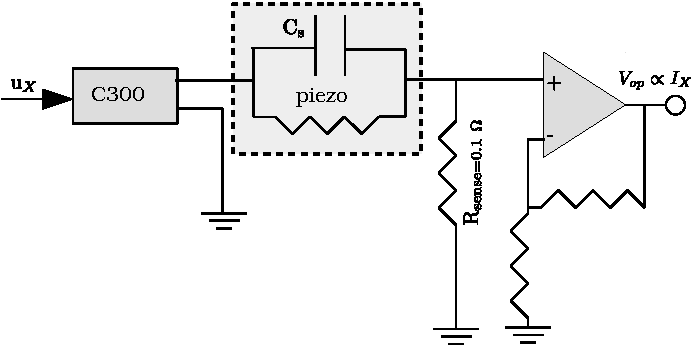
\includegraphics[width=1\columnwidth]{figures/blocks/c300_measurement_cropped.pdf}
    \caption{Schematic of the augmented current measurement used in characterizing the C300.}
    \label{fig:c300_meas}
  % \end{minipage}
\end{figure}
\section{System Modeling}
To keep the discussion manageable, we will concentrate the discussion to the $X$-direction. We model the overall plant for the $X$-direction as three cascaded systems: $\mathcal{F}$ which models the hysteresis of the piezo, a drift model $G_d$, and a vibrational model $\Gv$. This cascaded structure is shown in Fig.~\ref{fig:ss_bd}. In general, the effects of hysteresis are most noticeable when moving across wide ranges. Thus, by using relatively small input signals, the drift and vibrational dynamics can be identified separately from the hysteresis. Here, we model both $\Gv$ and $G_d$ as linear, time-invariant discrete-time systems. The dynamics of drift are predominantly low frequency while vibrational aspects on the other hand are fast by comparison, which allows the two systems to be easily separated in the identification.
 Modeling these three components is the subject of the next three subsections.


\subsection{Modeling \Gv}\label{sec:vib_model}
To obtain an experimental frequency response of $\Gv$, we use a stepped-sines method (single frequency at a time). The amplitude of the driving sinusoid is chosen to be small enough that the effects of hysteresis are minimized. After the system reaches steady-state, the input and output signals are demodulated into their first (complex) Fourier coefficients, the ratio of which yields the frequency response at that frequency. Fig.~\ref{fig:Guz2stage_frf} shows the resulting experimental FRF as the solid red curve.

\begin{figure}
  \centering
  \includesvg[width=01\linewidth]{figures/G_uz2stage_Eres.svg}
  \caption{The solid red curve is the frequency response from control input to stage position output in the $X$ direction. The dashed-black curve is the vibrational model, $\hat{G}_{\textrm{vib}}$.}
  \label{fig:Guz2stage_frf}
\end{figure}

Obtaining a parametric model of $\Gv$ for control design involves two steps. We obtain a preliminary model using an Eigenspace Realization Algorithm (ERA) \cite{Jacques_sysidfrf}. In general, the ERA does not produce a model with poles at $z=0$, which is what we need in order to model the delay. Thus, the delay in the frequency response is divided out of the FRF before passing it to the ERA algorithm.

The second step uses the model generated by the ERA as the initial guess to a non-linear least squares problem which minimizes the logarithm of the ratio of the experimental frequency response to that of the model~\cite{sidman_parametric_1991}. Though Sidman et al. develop the idea for continuous-time models, their strategy is easily adapted to fit a discrete-time model. In this scenario, the optimization is given by
\begin{align}
\min_{\theta} \sum_{i=1}^M\bigl| \log(G(e^{j\omega_iT_s})) - \log(\hat{G}(e^{j\omega_iT_s}|\theta))\bigr|^2
\label{eqn:logfit}
\end{align}
where $\omega_i$ is each frequency in the experimental frequency response and $\hat{G}(e^{j\omega_iT_s}|\theta)$ is the model parametrized by the vector $\theta$. The model $\hat{G}(z|\theta)$ is composed of first and second-order factors
\begin{equation}
  \hat{G}(z|\theta) =K \frac{\prod_{i=0}^{n_{rz}-1} (z-b^r_i) \prod_{j=0}^{n_{cz}-1}(z^2 +b^c_{2j}z + b^c_{2j+1})}
  { \prod_{\ell=0}^{n_{rp}-1}(z-a^r_\ell) \prod_{m=0}^{n_{cp}-1}(z^2 +a^c_{2m}z + a^c_{2m+1})}z^{-p} \label{eqn:mode_struc}
\end{equation}
where $n_{rz}$ and $n_{cz}$ (resp., $n_{rp}$ and $n_{cp}$) are the number of real and complex zeros (resp., poles) in the model generated by the ERA. The parameter vector $\theta$ is given by 
% \todo{Do you think this is too much detail here?}
\begin{equation}
\theta = [b^r_0\dots b^r_{n_{rz}}, b^c_{0}\dots b^c_{2n_{cz}-1}, a^r_0\dots a^r_{n_{rp}}, a^c_{0}\dots a^c_{2n_{cp}-1}, K, p].\nonumber
\end{equation}
Due to the logarithms in \eqref{eqn:logfit} and the multiplicative structure \eqref{eqn:mode_struc}, the Jacobian of $\log(\hat{G}(z|\theta))$ is surprisingly easy to calculate. Details can be found in \cite{sidman_parametric_1991}, though some modifications are required for the discrete-time case. 

The model structure \eqref{eqn:mode_struc} includes a fractional delay $z^{-p}$. This allows us to include the delay as a term in the decision variable and obviates the need to optimize over integers. This is further beneficial because we are not guaranteed that the latency from input to output is an exact integer multiple of the sample period and allowing a fractional delay helps the optimization to more accurately match the phase. In the final model, we round $p$ to the nearest integer. In this work, we do not model the modes above 1100~Hz. Thus, the optimization \eqref{eqn:logfit} is only done over frequency up to 1100~Hz. The final pole and zero locations for $\hGv$ are listed in Table \ref{tab:pzgvib}.

\begin{table}
  \caption{Pole and zero locations of $G_{\textrm{vib}}$. The graphic to the right shows their location (excluding the nine poles at $z=0$) in the $Z$-plane.}
  \label{tab:pzgvib}
  % \centering
  \begin{minipage}[T]{.6\linewidth}
    \small
  % \caption{Zero and pole locations of $\Gv$. }
    \input{Gvib_data.tex}
\end{minipage}% !important
% \hfill
\begin{minipage}[T]{.3\linewidth}
  \includesvg[scale=.8]{figures/pzplot.svg}
\end{minipage}
\end{table}


\subsection{Drift Modeling}\label{sec:drift_model}
% It is very common in the literature to fit a drift model to a single step input \cite{liu_creep_2013, croft_creep_1999}. This does not seem to be sufficient.
% It has been noted before in the literature that the rate of the creep affect itself is hysteretic \cite{Jung_open_loop_2000}, which I think in this context would imply that the real pole-zero pairs of $G_{drift}$ shift depending on the control history.
We model drift as the transfer function
\begin{equation}
\hat{G}_d(z|\theta) = \theta_5\frac{(z-\theta_1)(z-\theta_2)}{(z-\theta_3)(z-\theta_4)}.\nonumber
\end{equation}
Due to the comparatively slow dynamics of drift, it is more attractive to identify the drift model in the time domain rather than the frequency domain. 
We give the stage a step input with relatively small amplitude (to minimize the effects of hysteresis). The stage response is shown as the solid-blue curve in Fig.~\ref{fig:drift_fit}, while the simulated response of the vibrational model is shown as the dotted-black curve. The piezo drift is evident in the slow increase of stage position after the vibrational dynamics have decayed. 

\begin{figure}
  \includesvg[width=1\linewidth]{figures/drift_fit.svg}
  \caption{The stage is given a step input (dash-dotted black) with an amplitude of 0.15 volts, which results in the solid blue output trajectory. The response of the combined $\Gv$ and $G_{d}$ models is shown as the dashed red, while that of the vibrational model alone is the dotted black curve.}
  \label{fig:drift_fit}
\end{figure}
Let $\mathcal{Y}_{\text{exp}}$ represent the step response data collected from the stage and  $\mathcal{Y}_{\text{vib}}$ be the response of the model $\Gv$ to the same input. The goal then is to solve the non-linear least squares problem
% \todo{I think this is a bit awkward}
\begin{equation}
  \min_{\theta}\bigl|\bigl| \hat{g}_d(k|\theta)*\mathcal{Y}_{\text{vib}} - \mathcal{Y}_{\text{exp}}\bigr|\bigr|_2
  \label{eqn:fit_drift_cost}
\end{equation}
where $\hat{g}_d(k|\theta)$ is the impulse response corresponding to $\hat{G}_d(z|\theta)$, `$*$' represents the convolution operator, and  ${\theta=[\theta_1\dots\theta_5]}$ is the vector of parameters. To the extent that $\Gv$ accurately models the vibrational dynamics, the inclusion of $\mathcal{Y}_{\text{vib}}$ in \eqref{eqn:fit_drift_cost} effectively nullifies the vibrational aspects in the optimization. This is possible because, since we have a SISO system, $\Gv$ and $G_d$ commute. 
The non-linear optimization problem \eqref{eqn:fit_drift_cost} is solved with MATLAB's \texttt{lsqnonlin} and results in the red curve in Fig.~\ref{fig:drift_fit}, which shows the simulated step response of $\hat{G}_d\hGv$. 

\subsection{Hysteresis Modeling}\label{sec:hyst_model}
\begin{figure*}[h!]
  \begin{minipage}{0.48\textwidth}
  \includesvg[width=1\linewidth]{figures/hyst_response_ol.svg}
  \caption{The stage is driven by a sequence of filtered step inputs shown in the dotted black curve. The resulting stage response is the solid black curve, which shows good agreement, e.g., at the first step, but much worse agreement for larger steady-state values. The dashed red curve is the response of the overall combined model of $\hGv$, $\hat{G}_{d}$, and the complex hysteresis model $\mathcal{F}$.}
  \label{fig:hyst_resp_dem}
\end{minipage}
\hfill
\begin{minipage}{0.48\textwidth}
\centering
\includesvg[width=1\linewidth]{figures/G_pow_and_current.svg}
\caption{ The solid curve is the transfer function, $G_{I_X, u_X}$, from low voltage control to power amplifier output current, which is upper-bounded by the dotted and dashed curves, which represent a pure discrete derivative multiplied by the bounds \eqref{eqn:h1bound} and \eqref{eqn:duHinf}, respectively.}
\label{fig:powTF}
\end{minipage}
\end{figure*}

In typical raster scanning applications, hysteresis manifests as a bowing of the trajectory as the stage tries to track the linear ramps in a triangle wave (see, e.g., Fig. 3 of \cite{Leang_IEEECS_2009}). To motivate the need for hysteresis compensation in a step tracking application, consider Fig. \ref{fig:hyst_resp_dem}, which shows an input signal of various filtered steps applied open-loop to the stage. The solid black curve is the stage response, while the dotted-black curve is the input (scaled by the nominal DC-gain of $G_d\Gv$), which shows good agreement for the first step, but much worse agreement with the later steps, particularly those with large amplitudes. Effectively, the gain of the system depends on the control history, since for the same steady-state value of control, the steady-state value of the stage changes.

There are many models for hysteresis \cite{croft_creep_1999, rakotondrabe_bouc_2011, Lui_hysteresis_2013}. Here, we opt for simplicity (and by proxy, fast computation) and use the Modified Prandtl-Ishlinksi Hysteresis model developed in \cite{kuhnen_modeling_2003}. This hysteresis model is composed of a linear combination of saturation operators cascaded with a linear combination of classic hysteretic play\footnote{The term ``play'' is derived from the operator's use in modeling mechanical slop.} operators. The overall input-output relationship of the modified hysteresis operator $\mathcal{F}[\cdot]$ is
\begin{equation}
  \mathcal{F}(u_X) = w_s^T\mathbf{S}\left[w_H^T \mathbf{H}[u_X, z]\right]\nonumber
\end{equation}
where $\mathbf{S}$ and $\mathbf{H}$ are vectors of elementary saturation and play operators, respectively, and
where $w_s$ and $w_H$ are vectors of weights. The $i$th elementary play operator with associated threshold $d_H^i$, output $\xi_k^i$, and input $\nu_k$ is defined by the recursive relationship
\begin{align}
  \xi_k &=
  H^i(\nu_k|\: d_H^i) =
  \max\{\xi^i_{k-1}-d_H^i, \min\{\xi^i_{k-1} + d_H^i, \nu_k\} \}.\nonumber
\end{align}
% so that
% \begin{equation}
% \xi_k \triangleq w^T_H H[u_X,z] = w^T_H\begin{bmatrix}\xi_k^1&\dots&\xi_k^n\end{bmatrix}^T
% \end{equation}

In contrast, the saturation operator has no memory. The input-output relationship of the $i$th elementary saturation operator with associated threshold $d_S^i$ is defined as
\begin{align}
  \mu_k=
  S^i(\xi_k| d_S^i) &=
  \begin{cases}
    \max\{\xi_k - d_S^i, 0\} & d_S^i >0\nonumber\\
    \xi_k & d_S^i = 0\nonumber\\
    \min\{\xi_k-d_S^i, 0\},  & d_S^i<0.\nonumber
  \end{cases}
\end{align}
for an input $\xi_k$ and output $\mu_k$. 

If the thresholds $d_H^i$ and $d_S^i$ are pre-defined, \cite{kuhnen_modeling_2003} shows that it is possible to fit the weights $w_S$ and $w_H$ as the solution to a quadratic program. Using the input and output data shown in Fig.~\ref{fig:hyst_resp_dem}, we fit the weights $w_H$ and $w_S$ with several different numbers of operators. Though the quality of the fit increases with more operators, we found that the improvement did not increase substantially beyond 7 of each operator. 
The resulting fit with 7 saturation operators and 7 hysteresis operators is shown in Fig.~\ref{fig:hyst_resp_dem} as the dashed red curve (which also includes the drift and vibrational models). As the inset in that figure shows, it is possible to improve on this fit. One common alternative to cascading the drift and hysteresis models is to put them in parallel with each other \cite{mokaberi_compensation_2008, Krejci_inverse_2001}. While this does indeed lead to a smaller residual, it gives worse closed-loop performance than the present method.

\subsection{Power Amplifier Characterization and Limitations}\label{sec:powcharct}
The high voltage output of the C300 is current limited to 100 mA. The solid black curve in Figure~\ref{fig:powTF} shows the transfer function from the low voltage input of the C300 to current flowing through the stage, $G_{I_X,u_X}$, which is measured via the sensing resistor and op-amp shown in Fig~\ref{fig:c300_meas}. Because the piezo actuators are highly capacitive, at frequencies below about 600~Hz, $G_{I_X,u_x}$ looks like a pure derivative.
Thus, we can factor $G_{I_X,u_X}$ as
\begin{align}
  I_{X}(z) &= G_{I_X,u_X} u_X(z)\label{eqn:Gix_statebound}\\
          & = (z-1) G_o u_X(z)\nonumber\\
          & = G_o(z) \Delta u_X(z) \label{eqn:Gostatebound}
\end{align}
Ideally, one would enforce the current limit via a state-like constraint using \eqref{eqn:Gix_statebound} and a parametric model of $G_{I_X,u_X}$.
Although it is likely possible to solve such a problem with a high-end FPGA using, e.g., the Alternating Direction Method of Multipliers as developed in~\cite{Jerez_Trans_2014}, it is not possible to solve that problem on our hardware. Instead, we would like to approximate $G_o$ as a constant, which will lead to a box constraint on $\Delta u_X$. Thus, we need a bound $(\Delta u_k)_{\text{max}}$ such that
\begin{equation}
  |\Delta u_{X_k}| < (\Delta u_X)_{\text{max}} \implies |I_{\text{pow}}| < I_{\text{max}}.\label{eqn:du_bound0}
\end{equation}
It is straightforward to show that such a bound is given by 
\begin{equation}
(\Delta u_X)_{\text{max}} = \frac{I_{\text{max}}}{||g_o||_1}\label{eqn:h1bound}
\end{equation}
where $g_o$ is the impulse response of $G_o(z)$ and ${||g_o||_1 = \sum_{k=0}^{\infty}|g_o(k)|}$. The frequency response of this bound is shown in Fig. \ref{fig:powTF} as the dotted-black curve. In practice, we find that this bound is overly conservative. An alternative is to choose
\begin{equation}
(\Delta u_X)_{\text{max}} = ||G_o(z)||_{\infty}\approx 0.1980, \label{eqn:duHinf}
\end{equation}
which results in the dashed-black curve in Fig.~\ref{fig:powTF}. Although \eqref{eqn:duHinf} is only sufficient to guarantee \eqref{eqn:du_bound0} for sinusoidal inputs, in practice we find that enforcing \eqref{eqn:duHinf} does lead to the current staying under 100~mA.

% Notably, this bound is conservative, since for higher frequencies a pure derivative overestimates the amount of actual current draw. Ideally, we would use a parametric model of \(G_{I_{X},u_{X}}\) and enforce a constraint on the output of that model. However, such an approach renders the constraint set for $u_X$ complex and is it not feasible to solve that problem using the fast gradient method. In our experimental implementations, we will enforce \eqref{eqn:du_limit}.
% However, in Section~\ref{sec:time_save_analysis} we will consider how much performance is given up through this method via a simulation study. 

Finally, the slew-rate limit used in the MPC/linear feedback controller must be discounted from \eqref{eqn:duHinf} to account for the inverse drift compensator. This adjustment for the inverse drift operator follows essentially the same argument as above. We have
\begin{equation}
  (\Delta u)_{\text{max}} \leq \frac{(\Delta u_X)_{\text{max}}}{||G^{-1}_d(z)||_{\infty}} \approx 0.167 \label{eqn:du_discount}
\end{equation}
% \todo{should I say something about hysteresis inversion in the context}
\section{Control Setup}\label{sec:control_setup}
The constraint \eqref{eqn:du_discount} can be remodeled as a pure saturating constraint if we work with an incremental form of \(\Gv\) which has as its input \({\Delta u_k\coloneqq u_k-u_{k-1}}\), rather than \(u_k\). This is attractive because it not only allows us to directly penalize the rate of change in the optimal control problem but also renders the constraint \eqref{eqn:du_discount} as a box constraint on $\Delta u$, enabling the use of the computationally efficient Fast Gradient Method. Details on the form of the FGM we use can be found in \cite{Jerez_Trans_2014, jerez_embedded_2013} while specifics about our implementation are discussed in \cite{braker_application_2017}.
% \todo{Do you think I need to talk more about the FGM?}
% Putting a hard limit on $\Delta u$ in the linear feedback case is also simplified.
\subsection{The Incremental Form}\label{sec:incremental}
To develop the required incremental form, we augment the dynamics of \(\hGv=\{A,B,C,0\}\) with a state \(\x_{\text{u}}(k)\) such that
\begin{equation*}
  \x_{u_k} = u_{k-1}.\nonumber
\end{equation*}
It follows that
\begin{subequations}
\begin{align}
  % \begin{bmatrix}\x_{k+1}\\\x_{u_{k+1}}\end{bmatrix}
  \xd_{k+1}
  &=
    \begin{bmatrix}
      A & B\\ 0 & 1
    \end{bmatrix}
                  \xd_k
    % \begin{bmatrix}\x_k\\\x_{u_k}\end{bmatrix}
    +
    \begin{bmatrix}
      B\\1
    \end{bmatrix}
  \Delta u_k \label{eqn:deltadyn} \\
  \y_k & = \begin{bmatrix}C & 0\end{bmatrix}\xd_k\\
                              % \begin{bmatrix}\x_k\\\x_{u_k}\end{bmatrix}\\
    \xd_k& \coloneqq
    \begin{bmatrix}\x_k\\\x_{u_k} \end{bmatrix}
  % \xd(0) & = \begin{bmatrix}\x(0)\\u(-1)\end{bmatrix}. \label{eqn:x0_aug}
\end{align}\label{eqn:ssdelta}%
\end{subequations}
We call this system \(\Gd = \{\Ad, \Bd, \Cd, 0\}\), which has \({\bar{n}_s=23}\) states, 9 of which model delay.
To solve the setpoint tracking problem, we work in the error
coordinates of \(\Gd\).
For a constant reference \(r_{ss}\), in steady state we have \({\du_{ss}=0}\) and \({\xdss =N_{\xd}r_{ss}}\) where \({N_{\xd}\in\mathds{R}^{\bar{n}}}\) is found by solving
\begin{align}
  \begin{bmatrix}N_{\xd} \\ N_u\end{bmatrix} &=
\begin{bmatrix}I-\Ad & -\Bd\\\Cd & 0\end{bmatrix}^{-1}\begin{bmatrix}0\\ I\\\end{bmatrix}\label{eqn:nxnu},
\end{align}
which, due to the augmented pole at $z=1$, will give \(N_u\equiv 0\). 
The error state, \({\xd_{e_k}=\xd_k - \xdss}\) has dynamics
\begin{align}
  \xd_{e_{k+1}} & = \Ad\xd_k + \Bd\dd u_k - \xdss \nonumber\\
            & = \Ad \xd_{e_k}   + \Bd \dd u_k\nonumber
\end{align}
              because $\xdss$ is in the nullspace of $(I - \Ad)$.
              
\subsection{Observer Design}\label{sec:dist_est}
To achieve zero-offset tracking (to constant disturbances), we employ the disturbance estimator outlined in \cite{maeder_offset-free_2007}. The disturbance dynamics are modeled as a pure integrating disturbance. The estimator dynamics are then given by
\begin{align}
  \begin{bmatrix} \hat{\x}_{k+1}\\ \hat{d}_{k+1} \end{bmatrix}
  &= A_m
  \begin{bmatrix} \hat{\x}_{k}\\ \hat{d}_k\end{bmatrix}
    + B_m u_k + L_m(y_k - \hat y_k) \label{eqn:obsdyn}\\
  \hat y_k &= C_m\begin{bmatrix} \hat{\x}_k\label{eqn:yhat}\\
    \hat{d}_k \end{bmatrix}
\end{align}
where $\hat{x}$ is our estimate of $x_k$ (not $\bar{x}_k$), $\hat{d}_k$ is the disturbance estimate, and 
\begin{align}
  A_m& = \begin{bmatrix}
    A & B_d \\ 0 & 1
  \end{bmatrix},\:\:
  B_m =
  \begin{bmatrix}
    B \\ 0
  \end{bmatrix} \nonumber\\
  C_m &= 
    \begin{bmatrix}
    C & C_d
  \end{bmatrix},\:\:\;
  L_m = \begin{bmatrix} L_x\\L_d \end{bmatrix} \label{eqn:CmLm}
\end{align}
It is shown in \cite{maeder_offset-free_2007} that the gains $L_x$ and $L_d$ may be designed separately such that the closed-loop poles $A_m - L_mC_m$ are the same as $\sigma(A-L_xC)\cup \sigma(1-L_dC_d)$.
We set $L_x$ equal to the steady-state solution of the discrete LQR problem applied to the dual of $\hGv$, where $Q = \alpha BB^T$ and $\alpha$ is a tuning parameter. We design $L_d$ such that the disturbance pole is placed at $z=0.8$.

To achieve zero offset tracking, disturbance estimators re-compute the steady-state target $\xdss$ at each time-step. Here, we use an output disturbance model, so that $B_d=0$ and $C_d=I$, which means that the reference is adjusted by subtracting $\hat d_k$. In other words, at each time step, we need to compute
\begin{equation}
  \bar{x}_{e} =
  \begin{bmatrix}\hat{x}_k\\x_{u_k}
  \end{bmatrix}
  - N_{\bar{x}}(r_k - \hat{d}_k).\nonumber
\end{equation}
This is slightly simpler than the case for an input disturbance model ($C_d=0$ and $B_d\neq0$), which involves an additional vector-scalar multiplication and an additional vector-vector addition (see (21) in \cite{maeder_offset-free_2007}). It is shown in \cite{maeder_offset-free_2007} that output disturbance and input disturbance estimators are equivalent provided 1 is not an eigenvalue of $A$, which is the case here, because we do not estimate the state $x_u$. Thus, due to the computational savings, we use the output disturbance formulation. 
\subsection{Closed-Loop Equations}
Let us derive the closed-loop equations for the block diagram of Fig.~\ref{fig:ss_bd} with the drift and hysteresis operators set to the identity and with the controller given by a partitioned feedback gain ${K = [K_x\: K_u]}$. Similarly, the observer gain is partitioned as in \eqref{eqn:CmLm}.
In closed-loop we do not estimate $\x_u$, because it is perfectly known and we do not compute the state-feedback portion of the control with $\hat d$ because the disturbance is uncontrollable from $u_k$.  
From~\eqref{eqn:ssdelta}, \eqref{eqn:obsdyn} and \eqref{eqn:yhat} we have
\begin{align}
  \hat{\x}_{k+1} &= A \hat{x}_k + Bu_k + L_x(y_k - \hat{y}_k)\label{eqn:xhat}\\
  \hat{d}_{k+1}  &= \hat{d}_k  + L_d (y_k - \hat{y}_k) \label{eqn:dhat}\\
  x_{u_{k+1}}     &= x_{u_k}  + \Delta{u}_k,\label{eqn:xu}
\end{align}
where $y_k$ is the plant output. The control increment $\Delta u_k$ and control $u_k$ are given by
\begin{align}
  \Delta u_k &= -\begin{bmatrix}
    K_x & K_u
  \end{bmatrix}
  \begin{bmatrix}
    \hat{\x}_k \\ x_{u_k}
  \end{bmatrix}
  +
               \bar{N}(r_k - \hat{d}_k).\label{eqn:deltau}\\
  u_k &= \Delta u_k + x_{u_k}\label{eqn:uk}.
\end{align}
In \eqref{eqn:deltau}, $\bar{N}\triangleq KN_{\bar{x}}$ is the feedforward control gain, where $N_{\bar{x}}$ is defined by \eqref{eqn:nxnu}.
We can write \eqref{eqn:xhat}-\eqref{eqn:uk} as the combined state-space system
\begin{align}
\tilde{\x}_{k+1} &= \tilde{A}\tilde{\x}_k + \tilde{L}y_k + \tilde{B}\bar{N}r_k\label{eqn:cntrldyn}\\
u_k &= -\tilde{K}\tilde{\x}_k + \bar{N} r_k \label{eqn:ukx}
\end{align}
where
\begin{align*}
  \tilde{A} &= \begin{bmatrix}
    A-BK_x-L_xC & B(1-K_u) & -B\bar{N} - L_xC_d\\
    -K_x        & 1-K_u    & -\bar{N} \\
    -L_dC      & 0        & 1-L_dC_d
  \end{bmatrix}\\
  \tilde{L} &= \begin{bmatrix} L_x \\ 0 \\ L_d  \end{bmatrix},\:\:
  \tilde{B} = \begin{bmatrix} B \\ 1 \\0\end{bmatrix},\:\:
  \tilde{x}_k = \begin{bmatrix} \hat{x}_k \\ x_{u_k} \\ \hat{d}_k\end{bmatrix},\\
  \tilde{K} &= \begin{bmatrix}K_x & K_u-1 & \bar{N}\end{bmatrix},\\
\end{align*}
Taking the $\mathcal{Z}$-transform of \eqref{eqn:cntrldyn} and \eqref{eqn:ukx}, we obtain
\begin{align}
  u(z) =&  \bar{N}(1-\tilde{K}(zI-\tilde{A})^{-1}\tilde{B})r(z) \nonumber\\
       & -\tilde{K}(zI - \tilde{A})^{-1}\tilde{L}y(z).\label{eqn:uz}
\end{align}
If $G(z)$ (which need not be the same as our model $\Gv$) is the transfer function of the plant, then the $\mathcal{Z}$-transform of the output $y$ subject to an output disturbance $d$ and control input $u$ is $y(z) = G(z)u(z) + d(z)$. Combining this expression with \eqref{eqn:uz} we obtain 
\begin{align}
  y(z) &= \frac{G(z)\bar{N}(1-D_2(z))}{1 + G(z)D_1(z)} r(z) + \frac{1}{1 + G(z)D_1(z)}d(z)\label{eqn:cltf}
\end{align}
where
\begin{align*}
  D_1(z) &= \tilde{K}(zI -\tilde{A})^{-1}\tilde{L}\\
  D_2(z) &= \tilde{K}(zI -\tilde{A})^{-1}\tilde{B}.
\end{align*}
Thus, the loop gain is given by $L(z) = G(z)D_1(z)$ and we define the sensitivity function as
\begin{equation}
  \mathcal{S}(z)\triangleq \frac{1}{1+L(z)}.\label{eqn:Sens}
\end{equation}
Due to the disturbance estimator, $\mathcal{S}(z)$ will always have a zero at $z=1$ so that its DC-gain is zero. In Section~\ref{sec:results}, it will be helpful to quantify how large the sensitivity function gain is at small but non-zero frequencies. To this end, we define the ''integrated sensitivity''
\begin{equation}
\mathcal{S}_I(z)\triangleq \mathcal{S}(z)\frac{1}{z-1} \label{eqn:S_int}.
\end{equation}
The DC-gain of $\mathcal{S}_I(z)$ can then be used to quantify the low-frequency gain of $\mathcal{S}(z)$.

Recall that the closed-loop poles are the transmission zeros of $1+L(z)$ and are the union of the controller poles and observer poles, which can be seen through the separation principle or manipulation of the matrix pencil describing the transmission zeros. Moreover, in the first term of \eqref{eqn:cltf}, the observer poles are canceled by the transmission zeros of $(1-D_2(z))$. Of course, these properties only hold when the observer is a perfect model of the plant. The advantage in representing the closed-loop dynamics as \eqref{eqn:cltf} is that (1) it is perfectly valid when the observer and plant dynamics do not match and (2) it exposes cleanly how to analyze the robustness of our designs. 


% \begin{figure}
%   \includesvg[width=1\linewidth]{figures/obs_cl.svg}
%   \caption{(black) open-loop plant pole (x) and zero(circle) locations. (red x) closed-loop observer pole locations.}
%   \label{fig:obs_cl}
% \end{figure}


\section{Control Designs}\label{sec:tune}
\begin{figure*}
  % \begin{minipage}{0.48\textwidth} 
    \begin{subfigure}{0.48\textwidth}
  \includesvg[width=1\textwidth]{figures/lqr_locus_constsig_0p9.svg}
\caption{}
  \label{fig:lqr_locus_cs}
\end{subfigure}
\hfill
\begin{subfigure}{0.48\textwidth}
  \includesvg[width=1\textwidth]{figures/lqr_locus_choozezet.svg}
  \caption{}
  \label{fig:lqr_locus_cz}
\end{subfigure}
\caption{Root locus of closed-loop poles as a function of $\gamma$. Note that for clarity, the plant zeros are not shown. The black $\times$'s indicate the poles of the open-loop plant. The black circles indicate the fictitious zeros, which are at the location of the desired poles. (a) The constant-$\sigma$ scheme with $\sigma=0.9$. (b) The chosen-$\zeta$ scheme.}
\label{fig:lqr_locus}
\end{figure*}

%Both the MPC and linear state feedback controllers can be described by the optimization
Consider the optimal control problem
\begin{subequations}
\begin{align}
\min_{v}\:\:& z^T_{N}Pz_{N} + \sum_{i=0}^{N-1}z_{i}^{T}Qz_{i} + 2z^T_iSv_i + v^{T}_{i}Rv_{i} \label{eqn:optcost}\\
  % \text{s.t.}&\nonumber\\
  \text{s.t.}\:\:  z_{i+1} =& \Ad z_{i} + \Bd v_{i}\\
z_{0} =& [\hat{x}^T_{k}, x^T_{u_k}]^T - N_{\bar{x}}(r_k-\hat{d}_k)\\
|v_i | \leq& (\Delta u)_{\text{max}}.\label{eqn:cntrl_constraint}
\end{align}\label{eqn:optcon2}%
\end{subequations}
where $Q$ and $R$ are symmetric matrices and the matrices $Q,R,S$ satisfy \eqref{eqn:schur0} and \eqref{eqn:schur1}.
The terminal cost $P$ is the solution of the DARE. 

We consider two control strategies based on \eqref{eqn:optcon2}:
\par\noindent\emph{Constrained Model Predictive Control (MPC):} With this strategy, one solves \eqref{eqn:optcost} online, which results in a sequence of $N$ optimal controls, $\{v_i\}_{i=0}^{N-1}$.
One then sets $\Delta u_k = v_0$ and discards the remaining $v_i$. The process is repeated at the next time step. With MPC, the saturator in Fig.~\ref{fig:ss_bd} is superfluous because the optimal control satisfies the constraints by design. The goal with MPC is to directly account for the slew-rate constraint as part of the control law itself and hope that this results in increased performance.
% Due to limitations on the implementation, MPC must still be de-rated to some extent to be implementable, since the length of control horizon needed to achieve stabilty over the full range of the stage becomes large for an overly aggressive design.
% \item
\par\noindent\emph{Saturated Linear state feedback (SLF):}
Here, we eliminate the constraint \eqref{eqn:cntrl_constraint}. Thus,
\begin{equation*}
  \Delta u_k =v_0 = -Kz_0 %[\hat{x}^T_k, x_{u_k}]^T
\end{equation*}
where $K = (\Bd^TP\Bd + R)^{-1}(\Bd^TP\Ad + S^T)$,
which is the LQR feedback gain associated with $Q$, $R$, and $S$. 
In contrast to MPC, with SLF, the saturator in Fig.~\ref{fig:ss_bd} is necessary to avoid exceeding our current limit. While this scheme is much more computationally efficient than MPC, the fact that the constraint is not directly accounted for typically means that the performance requirements must be relaxed to maintain stability (e.g., by increasing the control weight $R$), due to the saturator.

In the next two subsections, we deal with the problem of designing the weighting matrices $Q$, $R$, and $S$.

\subsection{Control Weight Selection}
Let $Q = FF^T$ for some vector $F\in\mathds{R}^{\bar{n}_s}$, $S=F$, and $R=1+\gamma$ where $\gamma$ is a scalar parameter. Consider the fictitious output
\begin{equation}
  \eta_k = F^T\xd_k + v_k. \label{eqn:fictout}
\end{equation}
Then the running cost portion of \eqref{eqn:optcost} can be written as
\begin{equation}
   \sum_{i=0}^{N-1} \eta_i^T\eta_i + \gamma v_i^T v_i.
    % &= \sum_{i=0}^{N-1} \hat{x_i}^TQ\hat{x_i} + 2x_i^TSu_i + u_i^T(R_o+\gamma)u_i
\end{equation}
As the control weight $\gamma$ becomes small, the closed-loop poles of the unconstrained LQR
will move to the zeros of $\{A, B, F^T, 1\}$. This is illustrated in Fig.~\ref{fig:lqr_locus} for two different $F$ vectors (discussed further later in this subsection). Thus, we can effect pole-placement through the proper design of $F$ and by taking $\gamma$ to be small.
With this selection of $Q$ and $S$, \eqref{eqn:schur1} becomes
\begin{equation}
FF^T\left(1 - \frac{1}{1+\gamma} \right)\geq 0
\end{equation}
which holds for all $\gamma\geq 0$. However, numerical difficulties tend to arise in computing $P$ when $\gamma$ is too close to zero. Nonetheless, one can usually take $\gamma$ to be small enough that the difference between the desired pole locations and their actual locations is negligible. The direct feedthrough in \eqref{eqn:fictout} results in the cross-weighting term $S$ and is necessary if we wish to endow the fictitious system with $\bar{n}_s$ zeros in order to place all $\bar{n}_s$ poles.

Through elementary block row and column operations, it is straightforward to show that the zeros of
$\{A, B, F^T, 1\}$ are the same as the solutions of the generalized eigenvalue problem
\begin{equation*}
  \begin{bmatrix}
    (A - BF^T) & 0\\
    0 & 1
  \end{bmatrix} - \begin{bmatrix}zI & 0\\0 & 0\end{bmatrix} = 0.
\end{equation*}
Thus, one may find $F$ via standard pole placement techniques.

Certainly, in the case of the SLF state feedback controller, one could simply use a pole-placement design to start with. However, the method here has two advantages: (1) it permits a straightforward comparison to the MPC design (which, in the present formulation, requires weighting matrices, not simple pole locations) and (2) the design becomes parametrized by the scalar parameter $\gamma$ which makes de-rating the design easy. In contrast, with standard pole-placement, it is not clear how to ``back-off'' the design if the slew-rate constraint is violated to the extent that instability results. 

% \subsection{Selecting Desired Poles}
We consider two methods to choose a set of desired pole locations. The first method we call ``constant-$\sigma$'' (CS). The idea is to move all complex poles such that they lie on a circle with a specified radius, which endows them all with the same time constant. Here, we select the radius as $\sigma=0.9$.

The second scheme, which we call ``choose-$\zeta$'' (CZ), keeps the natural frequency of each complex pole unchanged but specifies a damping ratio $\zeta$. As we will see in the next section, this approach generally yields slower settling time than the constant-$\sigma$ method: however it tends to result in slightly smaller residual oscillations and is the same scheme we considered previously in \cite{braker_fast_2017, braker_application_2017}, so we include it here so that these results can be evaluated in light of our prior work.

For both cases, we place the 9 poles corresponding to the delay at the roots of unity with a radius chosen more less arbitrarily at ${\sigma=0.25}$. Fig.~\ref{fig:lqr_locus} shows root locus-like plots for each scenario as a function of $\gamma$. As $\gamma$ approaches zero, the closed-loop poles approach the designed fictitious zeros, which are indicated by black circles. 

\subsection{Selecting $\gamma$}
The choice of $\gamma$ has a significant effect on system performance. Because this effect differs between simulation and experiment, we explore that aspect of the tuning in the next section.

\section{Simulated vs Experimental Performance and Dependence on $\gamma$}\label{sec:results}
\begin{figure}[ht!]
  \includesvg[scale=1]{figures/steps.svg}
  \caption{The sequence of step commands used to test the control laws. The red circles indicate the 5th and 24th reference. The response to these references are shown in closer detail in Fig.~\ref{fig:min_gam_traj} and \ref{fig:rob_gam_traj}.}
  \label{fig:steps}
\end{figure}
The goal of this section is to explore how the simulation and experimental performance of MPC and SLF (for both pole placement schemes) depends on the control weight $\gamma$ and to determine to what extent, if any, MPC provides a benefit.

We tested the experimental and simulation performance of the SLF and MPC control schemes using 
a sequence of 24 reference commands. The first 20 references we selected randomly within the range $[-32.5~\mu$\text{m}, $35\mu\text{m}]$. We chose the final four references as $0~\mu$m, $35~\mu$m, $-32.5~\mu$m, and $0~\mu$m, to exercise the full usable range of the stage\footnote{For a references larger 35~$\mu$m, the control signal saturates; for references smaller than -32.5~$\mu$m, the sensor saturates due to a bias in the stage.}. This sequence of references is shown in Fig.~\ref{fig:steps}. Using a sequence of randomly generated references (rather than, e.g., a single reference or several references beginning from rest) has several benefits: (1) it is representative of the type of references seen in a compressive sensing imaging scenario \cite{braker_hardware_2018}; (2) it eliminates the possibility of cherry picking specific reference values where one control law does better and (3) using a \emph{sequence} of references will help to draw out the deleterious affects of imperfections in the hysteresis and drift inversion.

To explore the performance dependence on $\gamma$, we ran a series of experiments and simulations across a grid of $\gamma$'s ranging from $\gamma=10^{-5}$ to $\gamma=400$. 
Each simulation was run once and each experiment was conducted 8 times. 
We define the settling time in an absolute sense. Specifically, the settle boundary is 70~$\mu$m/512, which corresponds to settling within one pixel of a 512 by 512 pixel image for the given range.
Let $t_i^j(\gamma_{\ell})$ represent the settling time of the $i$th reference for the $j$th experimental run using the $\ell$th $\gamma$ in our grid. Then the total settling time of the $j$th experiment is $T_j = \sum_{i=1}^{24} t_i^j(\gamma_{\ell})$. The sample mean of the total settling times for a specific $\gamma_{\ell}$ is
\begin{equation}
  \bar{T}(\gamma_{\ell}) = \frac{1}{8}\sum_{j=1}^8 T_j(\gamma_{\ell}).
\end{equation}


Fig.~\ref{fig:GainS} plots the mean of the total experimental settling times (i.e., $\bar{T}(\gamma_{\ell})$) vs $\gamma$ as the red (MPC) and black (SLF) dots with error bars. The left panel shows the results for the CS scheme and right panel shows the results for the CZ scheme. Note that the SLF experiments and simulations are not run with the smallest values of $\gamma$ because they become unstable.
The simulation settling times are shown in Fig.~\ref{fig:BW}. Here, the MPC simulations are indicated by the red circles and the SLF simulations are indicated by the black dots.
For reference, the actual values of the plotted data are shown in Table~\ref{tab:CS_ts_total} and \ref{tab:CZ_ts_total}. 

For the smallest tested values of $\gamma$, Fig.~\ref{fig:min_gam_traj} shows zoomed-in experimental trajectories of the four controllers for references 5 and 24 (circled in Fig.~\ref{fig:steps}). The fastest experimental settling times occur for $\gamma=100$ for the CS scheme and $\gamma=25$ for the CZ scheme. Zoomed-in experimental trajectories for these values of $\gamma$ are shown in Fig.\ref{fig:rob_gam_traj}, also for references 5 and 24.

For all of the experimental trajectories, the largest measured power amplifier current was 98.5~mA, indicating success in respecting the 100~mA current limit.

\subsection{Discussion}\label{sec:res_disc}
In both simulation and experiment MPC is able to utilize a much smaller $\gamma$ than SLF. In the simulation results, increasing $\gamma$ results in an increased total settling. This is as one would expect, because nominal closed-loop bandwidth decreases as $\gamma$ increases, as shown by the solid black curves in Fig.~\ref{fig:BW}. Interestingly, this trend does not hold in the experimental results. Up to about ${\gamma=100}$ for CS and ${\gamma=25}$ for CZ, total settling time settling time \emph{decreases} as $\gamma$ increases in the experimental results. This means, e.g., that when ${\gamma=10^{-5}}$ in the CZ MPC experiment, the total settling time is nearly 3 times slower than the simulation; when ${\gamma=25}$ the experiment is only 1.3 times slower than simulation.

These trends can be explained by analyzing how robustness depends on $\gamma$. First, recall from Sections~\ref{sec:drift_model} and \ref{sec:hyst_model} that our overall control loop inverts imperfect models of hysteresis and drift. Errors in these inversions will show up as model uncertainty at low frequencies. Thus, we expect that when the gain of the sensitivity function at low frequencies is small, then the effect of these uncertainties will be reduced. To quantify how the low-frequency gain of $\mathcal{S}$ (which is always zero at DC) depends on $\gamma$, we computed the DC-gain of the integrated sensitivity function $\mathcal{S}_I$, defined in \eqref{eqn:S_int}, at a grid of $\gamma$s. The resulting parametric plot is shown as the black curves in Fig.~\ref{fig:GainS}, which are plotted against the right axes. Notably, the decrease and subsequent increase in total settling time roughly follows the DC-gain of $\mathcal{S}_I(z)$ vs $\gamma$ curve.

A complementary analysis is to consider how the GM and PM change as $\gamma$ increases. Parametric plots of these metrics (computed from the loop gain $L(z)$) are shown in Fig.~\ref{fig:gmpm}. 
Here, we see that for both pole-placement scenarios, robustness in terms of GM and PM increases monotonically as $\gamma$ increases and is quite poor for the smallest values of $\gamma$.
% The negative PM for the CZ scenario is due to an unstable pole in $L(z)$. 

\begin{table*}
  \caption{Total settling times for (a) the constant-$\sigma$ and (b) chooze-$\zeta$ state weighting schemes. The second and third columns of each table are the simulation results while the fourth and fifth columns are the average of 8 experimental runs. SLF was not run for the smallest $\gamma$ values, as indicated by the dashes. All times are in milliseconds.}
  \begin{minipage}{1\textwidth}
  \begin{subtable}{0.5\textwidth}
    \caption{Constant-$\sigma$}
    \scriptsize
  \begin{tabular}{ccccc}
    \input{ts_means_CS.tex}
    \label{tab:CS_ts_total}
  \end{tabular}
\end{subtable}
\hfill
\begin{subtable}{0.5\textwidth}
  \caption{Choose-$\zeta$}
  \begin{tabular}{ccccc}
    \scriptsize
    \input{ts_means_CZ.tex}
    \label{tab:CZ_ts_total}
  \end{tabular}
\end{subtable}
\end{minipage}
\begin{minipage}{1\textwidth}
  \vspace{1em}
  \includesvg[scale=1]{figures/GainS_TS_vs_gamma_both.svg}
  \captionof{figure}{(left) constant-$\sigma$. (right) chooze-$\zeta$. The black (SLF) and red (MPC) dots with error bars are the sample means of the total settling times for different values of $\gamma$ and are plotted against the left axes. The solid black curve is DC-gain of the integrated sensitivity function $\mathcal{S}_I(1)$ evaluated at different values of $\gamma$, plotted against the right axes.}
  \label{fig:GainS}
\end{minipage}
\begin{minipage}{1\textwidth}
  \vspace{1em}
  \includesvg[scale=1]{figures/BW_TS_vs_gamma_both.svg}
  \captionof{figure}{(left) constant-$\sigma$. (right) chooze-$\zeta$. The red circles (MPC) and black dots (SLF) are the total simulated settling times for different values of $\gamma$ and a plotted against the left axis. The solid black curve is the closed-loop 3~dB closed-loop bandwidth evaluated for different values of $\gamma$, plotted against the left axis.}
    \label{fig:BW}
\end{minipage}  
\end{table*}
\begin{figure*}[h!]
  \begin{subfigure}{1\columnwidth}
    \includesvg[width=1\columnwidth]{figures/step_exps_min_gam.svg}
    \caption{
      % Experimental trajectories for the constant-$\sigma$ and chosen-$\zeta$ pole placement schemes. The two columns zoom in on the two responses indicated by the red ellipses in Fig.~\ref{fig:steps}. (first row) Stage output trajectories. The dotted-black lines indicate the settle boundary. (second row) Control increment trajectories. 
      % The abbreviations in the legend are defined in Table~\ref{tab:gmpms}.
    }
  \label{fig:min_gam_traj}
\end{subfigure}
\hfill
% \end{figure}
% \begin{figure}
\begin{subfigure}{1\columnwidth}
  \includesvg[width=1\columnwidth]{figures/step_exps_rob_gam.svg}
  \caption{
    % Experimental trajectories for the choose-$\zeta$ pole placement scheme. The top panel shows all 24 step responses. The two columns zoom in on the two responses indicated by the red ellipses. (second row) Stage output trajectories. The dotted-black lines indicate the settle boundary. (third row) Control increment trajectories. (fourth row) Measured power amplifier current. The abbreviations in the legend are defined in Table~\ref{tab:gmpms}.
  }
  \label{fig:rob_gam_traj}
\end{subfigure}
\caption{Stage output (top row) and control increment (bottom row) experimental trajectories for references 5 and 24 (circled in Fig.~\ref{fig:steps}). (a) Trajectories for the smallest tested values of $\gamma$. (b) Trajectories for the values of $\gamma$ resulting in the fastest total experimental settling time.}
\end{figure*}

Ultimately, the experimental fastest settling time which we can acheive for either pole-placement scenario is a trade-off between the robustness metrics  GM, PM and $\mathcal{S}_I(1)$ and the nominal (i.e., simulated) increase in settling time as $\gamma$ increases. Determining the precise nature of this trade-off would require precise knowledge of the model uncertainty, which is unknown. Moreover, for the fastest experimental settling times (i.e., ${\gamma=100}$ for CS and ${\gamma=25}$ for CZ) the difference in trajectories and thus total settling times between MPC and SLF is negligible. The close correspondence of MPC and SLF trajectories for large $\gamma$ is illustrated in Fig.~\ref{fig:rob_gam_traj} for references 5 and 24. The similarity in total settling times between MPC and SLF holds for both simulation and experiment as can be seen in the ${\gamma=100}$ row of Table~\ref{tab:CS_ts_total} and the ${\gamma=25}$ row of \ref{tab:CZ_ts_total}. We conclude that, under the present state weighting schemes, input constrained MPC provides no additional benefit.


\subsection{Possible Objections}
We envision three main criticisms to these results and analysis. First, one might rightly point out that both MPC and SLF are in general, non-linear making the classical metrics like PM, GM and $|\mathcal{S}_I(1)|$ inapplicable. However, for any setpoint, both SLF and MPC behave linearly in a neighborhood around that setpoint. In other words, while the beginning of a setpoint tracking maneuver may saturate the SLF controller or put the MPC on its constraint boundary, the latter part of that same maneuver will be governed by linear dynamics. In that sense, the metrics GM and PM and the DC-gain of the integrated sensitivity still provide some insight, which we believe is manifested, e.g., in the correlation between overall settling time and $|\mathcal{S}_I(1)|$.

A related objection is that the relatively poor GMs and PMs could be improved through a loop transfer recovery (LTR) method. However, the classic method as proposed in \cite{doyle_robustness_1979} does not translate directly to discrete-time. Most efforts at obtaining LTR-like results for discrete-time assume that (1) a current estimator is used and (2) $CB\neq 0$ \cite{Maciejowski_asymptotic_1985,guaracy_discrete_2015,ishihara_loop_1986}. When considering MPC, especially at high sample rates, we need to use a prediction estimator, since computing the control action requires a significant portion of the sample period. Also, for our system model, $CB=0$, because the relative degree is 12. These two factors preclude discrete-time LTR. Even if these issues could be circumvented, we must bear in mind that, in contrast to the continuous-time case, the full-state feedback discrete-time LQR controller does not have a guaranteed infinite gain margin nor a guaranteed phase margin greater than $60^{\circ}$. Rather, the guaranteed bounds for GM and PM depend on the DARE solution $P$~\cite[p. 136]{andersson_moore}, which in turn depends on $\gamma$. 

Finally, one might argue that if we implemented time-optimal MPC (TOMPC) \cite{broeck_time_2009} instead of MPC with a purely quadratic cost, then MPC might show some benefit. Unfortunately, TOMPC requires the solution of a \emph{sequence} of optimal control problems with long horizons at each time step \cite{broeck_time_2009}. Thus, despite the advances in hardware and algorithms, such methods remain too slow for systems with fast dynamics. 

\begin{figure}[ht!]
  \includesvg[scale=.9]{figures/PMGM_vs_gamma_both.svg}
  \caption{GM and GM dependence on $\gamma$.}
  \label{fig:gmpm}
\end{figure}

\section{Conclusions}
% However, despite modeling and compensating drift and hysteresis, model uncertainty negated any gains
% We have compared the performance of an MPC and saturated linear feedback controllers, augmented with inverse compensators for hysteresis and drift. 
In this paper we have given an account of developing a setpoint tracking control law for a piezo stage, subject to a current limitation in the piezo power amplifier. To account for this current limit, we developed an incremental form with $\Delta u_k$ as its control input and showed that, by conservatively constraining $\Delta u_k$, we could keep power amplifier current within the 100~mA limitation. To this end, we developed MPC and saturated linear feedback control laws designed with two separate state weighting schemes. In agreement with our earlier work~\cite{braker_application_2017}, our MPC controllers were able to utilize a more aggressive control weight.

By considering the closed-loop performance across a wide range control weights, we showed that the aggressive weights (where MPC nominally provides some benefit), actually result in worse experimental performance in terms of settling time. We argued that this surprising result is due to model uncertainty and showed that closed-loop robustness degrades with small control weights. 

It is possible that MPC could be beneficial if, rather than constraining the slew rate of the low-voltage input, we constrained the output of a power amplifier current model. Such an MPC problem could no longer be solved with the FGM, though with a much larger FPGA, it may be possible that the problem could be solved with the Alternating Direction Method of Multipliers (ADMM) \cite{Jerez_Trans_2014}. Such an alternative formulation would only change the constraints, not the cost. Thus, the robustness properties explored in this paper would remain unchanged, though it is possible they would play a smaller role. However, embedded platforms with FPGAs capable implementing the ADDM at the required sample rate remain expensive. Thus, even if the state constrained problem could improve performance over SLF, this improvement would need to be weighed against the cost of simply upgrading the power amplifier. 

% As we noted in Section~\ref{sec:powcharct}, a slew rate constraint on the low-voltage input is conservative. An alternative would be to formulate the optimal control problem such that the output of the power amplifier current model was constrained. Such an MPC problem could no longer be solved with the FGM, though with a larger FPGA the problem could be solved with the Alternating Direction Method of Multipliers (ADMM) \cite{Jerez_Trans_2014}. Although the ADMM represents a substantial increase in both hardware requirements and code complexity, it is possible that MPC would be beneficial in that case. However, such an alternative formulation would only change the constraints, not the cost. Thus, the robustness properties explored in this paper would remain unchanged. Moreover, embedded platforms with FPGAs capable implementing the ADDM remain expensive. Thus, even if the state constrained problem could improve performance over SLF, this improvement must be weighed against simply upgrading the power amplifier. 

% On the other hand, despite the impressive recent advances in FPGA-based QP solvers, computing a linear feedback law will always yield a significantly faster achievable sample rate. Moreover, it has been shown that continuous-time robustness properties are recovered in the limit as the sampling frequency approaches 0. Thus, while in this paper we have compared MPC and linear feedback using the same sampling frequency, an interesting line for further investigation is: How much does robustness increase when the sampling frequency increases?

% We will show that in simulation, this idea does indeed lead to a significantly decreased settling time. However, the desire to decrease $\gamma$ must be tempered by its affect on both robustness and disturbance rejection, because these things are a metric for how the control will perform in practice. Unfortunately, we will see that decreasing $\gamma$ tends to degrade both properties for the weighting matrices we consider. 


\bibliographystyle{IEEEtran}
\bibliography{/home/arnold/bib_pdf/main_bibliography.bib}


\end{document}